\subsection{Experiment One: Best Input Combination}

\subsubsection{Best Input Combination Results}
\label{sec:simpleInputTest}
The simple input test based on 3 month historical data and 200 epochs.

WS = Wind Speed
AD = Air Density
C = Consumption
T = Temperature
WD = Wind Direction
L-P = Last Known Production
D = Date
ToD = Time of Day
M = Time of Day as matrix
CD = Correct Direction

\footnotesize
\begin{center}
\begin{longtable}{|c|c|c|c|c|c|c|c|c|c|c|c|c|}
\caption{Wind Production Input Parameter Test}\\
\hline
\textbf{WS} & \textbf{AD} & \textbf{C} & \textbf{T} & \textbf{WD} & \textbf{L-P} & \textbf{D}& \textbf{ToD} & \textbf{MAE} & \textbf{\% from \#1} & \textbf{H1} & \textbf{H2} & \textbf{CD} \\
\hline
\endfirsthead
\multicolumn{13}{c}%
{\tablename\ \thetable\ -- \textit{Continued from previous page}} \\
\hline
\textbf{WS} & \textbf{AD} & \textbf{C} & \textbf{T} & \textbf{WD} & \textbf{L-P} & \textbf{D}& \textbf{ToD} & \textbf{MAE} & \textbf{\% from \#1} & \textbf{H1} & \textbf{H2} & \textbf{CD}  \\
\hline
\endhead
\hline \multicolumn{13}{r}{\textit{Continued on next page}} \\
\endfoot
\hline
\endlastfoot
\arrayrulecolor{light-gray}
 \x &  &  &  \x &  &  \x &  &  \x & 125,75 & 0,0\% & 19 & 13 & 73\% \\ \hline
 \x &  \x &  &  &  \x &  \x &  &  \x & 131,59 & 4,64\% & 20 & 17 & 73\% \\ \hline
 \x &  \x &  &  &  &  \x &  &  \x & 131,89 & 4,88\% & 16 & 20 & 73\% \\ \hline
 \x &  \x &  \x &  \x &  \x &  \x &  &  \x & 133,18 & 5,91\% & 13 & 20 & 72\% \\ \hline
 \x &  \x &  \x &  \x &  \x &  \x &  &  \x & 133,77 & 6,38\% & 16 & 17 & 73\% \\ \hline
 \x &  \x &  \x &  &  &  \x &  &  \x & 134,14 & 6,67\% & 12 & 17 & 73\% \\ \hline
 \x &  \x &  \x &  &  \x &  \x &  &  \x & 135,4 & 7,67\% & 6 & 13 & 72\% \\ \hline
 \x &  \x &  \x &  &  &  \x &  &  \x & 136,33 & 8,41\% & 21 & 10 & 73\% \\ \hline
 \x &  \x &  &  &  &  \x &  \x &  \x & 136,65 & 8,67\% & 5 & 24 & 73\% \\ \hline
 \x &  &  &  &  &  \x &  &  \x & 137,33 & 9,21\% & 9 & 15 & 74\% \\ \hline
 \x &  &  &  \x &  \x &  \x &  &  \x & 137,8 & 9,58\% & 17 & 16 & 73\% \\ \hline
 \x &  \x &  &  &  \x &  \x &  &  \x & 138,16 & 9,87\% & 15 & 21 & 72\% \\ \hline
 \x &  &  \x &  &  &  &  &  \x & 138,33 & 10,0\% & 23 & 13 & 64\% \\ \hline
 \x &  \x &  &  \x &  &  \x &  &  \x & 138,94 & 10,49\% & 10 & 25 & 72\% \\ \hline
 \x &  \x &  &  &  &  &  &  \x & 139,25 & 10,74\% & 23 & 12 & 54\% \\ \hline
 \x &  \x &  &  &  &  \x &  &  \x & 139,35 & 10,82\% & 16 & 14 & 73\% \\ \hline
 \x &  \x &  \x &  &  &  &  &  \x & 139,67 & 11,07\% & 17 & 20 & 64\% \\ \hline
 \x &  &  \x &  &  \x &  \x &  &  \x & 139,78 & 11,16\% & 21 & 9 & 71\% \\ \hline
 \x &  \x &  \x &  \x &  &  &  &  \x & 139,99 & 11,32\% & 11 & 19 & 64\% \\ \hline
 \x &  &  &  &  &  &  &  \x & 140,14 & 11,44\% & 16 & 9 & 41\% \\ \hline
 \x &  &  &  &  \x &  &  &  \x & 140,44 & 11,68\% & 17 & 20 & 61\% \\ \hline
 \x &  &  &  \x &  &  \x &  &  \x & 140,55 & 11,77\% & 13 & 13 & 73\% \\ \hline
 \x &  &  \x &  &  &  \x &  &  \x & 140,82 & 11,98\% & 18 & 16 & 73\% \\ \hline
 \x &  \x &  \x &  &  &  &  &  \x & 140,85 & 12,01\% & 16 & 18 & 64\% \\ \hline
 \x &  \x &  \x &  \x &  &  \x &  &  \x & 140,91 & 12,06\% & 18 & 13 & 73\% \\ \hline
 \x &  \x &  &  &  &  &  &  \x & 141,09 & 12,2\% & 23 & 9 & 53\% \\ \hline
 \x &  &  \x &  &  &  &  &  \x & 141,28 & 12,35\% & 19 & 15 & 64\% \\ \hline
 \x &  &  \x &  &  \x &  &  &  \x & 141,38 & 12,43\% & 16 & 22 & 65\% \\ \hline
 \x &  &  &  &  \x &  &  &  \x & 141,5 & 12,52\% & 18 & 1 & 60\% \\ \hline
 \x &  &  &  &  \x &  \x &  &  \x & 142,22 & 13,1\% & 21 & 9 & 72\% \\ \hline
 \x &  \x &  \x &  \x &  &  \x &  \x &  \x & 142,35 & 13,2\% & 5 & 20 & 72\% \\ \hline
 \x &  \x &  &  \x &  \x &  &  &  \x & 142,44 & 13,27\% & 2 & 23 & 61\% \\ \hline
 \x &  \x &  \x &  &  &  \x &  \x &  \x & 142,57 & 13,38\% & 15 & 14 & 73\% \\ \hline
 \x &  \x &  &  \x &  &  \x &  &  \x & 142,64 & 13,43\% & 17 & 20 & 72\% \\ \hline
 \x &  &  \x &  &  &  \x &  &  \x & 142,67 & 13,46\% & 18 & 13 & 72\% \\ \hline
 \x &  \x &  \x &  &  \x &  &  &  \x & 142,75 & 13,52\% & 18 & 18 & 63\% \\ \hline
 \x &  &  \x &  \x &  \x &  \x &  &  \x & 142,97 & 13,69\% & 25 & 12 & 71\% \\ \hline
 \x &  \x &  &  &  \x &  &  &  \x & 143,07 & 13,77\% & 2 & 24 & 61\% \\ \hline
 \x &  \x &  \x &  &  &  &  \x &  \x & 143,23 & 13,9\% & 6 & 25 & 64\% \\ \hline
 \x &  &  \x &  \x &  &  \x &  &  \x & 143,24 & 13,91\% & 20 & 9 & 72\% \\ \hline
 \x &  \x &  &  \x &  &  &  &  \x & 143,53 & 14,14\% & 21 & 10 & 54\% \\ \hline
 \x &  \x &  &  &  \x &  &  &  \x & 143,98 & 14,5\% & 17 & 14 & 61\% \\ \hline
 \x &  \x &  \x &  &  \x &  &  &  \x & 144,06 & 14,56\% & 12 & 21 & 63\% \\ \hline
 \x &  \x &  \x &  &  &  \x &  \x &  \x & 144,24 & 14,7\% & 25 & 10 & 71\% \\ \hline
 \x &  &  &  \x &  \x &  \x &  &  \x & 144,95 & 15,27\% & 12 & 20 & 72\% \\ \hline
 \x &  \x &  \x &  &  \x &  \x &  &  \x & 144,96 & 15,28\% & 9 & 18 & 71\% \\ \hline
 \x &  &  &  &  &  \x &  &  \x & 145,11 & 15,4\% & 18 & 13 & 72\% \\ \hline
 \x &  \x &  &  \x &  \x &  \x &  &  \x & 145,26 & 15,51\% & 16 & 19 & 72\% \\ \hline
 \x &  \x &  \x &  \x &  &  &  &  \x & 145,49 & 15,7\% & 2 & 23 & 65\% \\ \hline
 \x &  &  \x &  &  \x &  \x &  \x &  \x & 145,92 & 16,04\% & 9 & 22 & 73\% \\ \hline
 \x &  &  \x &  &  \x &  &  \x &  \x & 145,98 & 16,09\% & 11 & 18 & 64\% \\ \hline
 \x &  &  \x &  &  &  &  \x &  \x & 146,01999999999998 & 16,12\% & 16 & 16 & 64\% \\ \hline
 \x &  \x &  \x &  \x &  &  &  \x &  \x & 146,32 & 16,36\% & 16 & 9 & 64\% \\ \hline
 \x &  &  \x &  \x &  &  &  &  \x & 146,48 & 16,49\% & 20 & 17 & 64\% \\ \hline
 \x &  &  \x &  &  \x &  &  &  \x & 146,82 & 16,76\% & 15 & 19 & 64\% \\ \hline
 \x &  \x &  &  &  &  &  \x &  \x & 147,08 & 16,96\% & 1 & 25 & 54\% \\ \hline
 \x &  &  &  \x &  &  &  &  \x & 147,41 & 17,22\% & 21 & 1 & 51\% \\ \hline
 \x &  \x &  &  \x &  \x &  \x &  \x &  \x & 147,99 & 17,69\% & 15 & 19 & 72\% \\ \hline
 \x &  \x &  \x &  \x &  &  \x &  \x &  \x & 148,27 & 17,91\% & 20 & 10 & 72\% \\ \hline
 \x &  &  \x &  \x &  \x &  \x &  &  \x & 148,61 & 18,18\% & 24 & 10 & 71\% \\ \hline
 \x &  &  &  \x &  \x &  &  &  \x & 148,67 & 18,23\% & 13 & 22 & 60\% \\ \hline
 \x &  &  &  \x &  &  &  &  \x & 149,27 & 18,7\% & 14 & 19 & 51\% \\ \hline
 \x &  &  &  &  &  &  &  \x & 149,72 & 19,06\% & 9 & 25 & 41\% \\ \hline
 \x &  &  \x &  &  &  &  \x &  \x & 149,8 & 19,13\% & 22 & 14 & 64\% \\ \hline
 \x &  \x &  \x &  \x &  &  \x &  &  \x & 149,85 & 19,17\% & 25 & 10 & 71\% \\ \hline
 \x &  &  &  &  &  \x &  \x &  \x & 150,3 & 19,52\% & 13 & 20 & 72\% \\ \hline
 \x &  \x &  \x &  \x &  &  &  \x &  \x & 150,45 & 19,64\% & 22 & 16 & 64\% \\ \hline
 \x &  &  \x &  \x &  \x &  &  &  \x & 150,63 & 19,79\% & 14 & 24 & 63\% \\ \hline
 \x &  &  \x &  \x &  &  \x &  &  \x & 150,96 & 20,05\% & 14 & 13 & 71\% \\ \hline
 \x &  &  \x &  &  \x &  \x &  &  \x & 151,54 & 20,51\% & 14 & 18 & 71\% \\ \hline
 \x &  &  &  &  \x &  \x &  &  \x & 151,55 & 20,52\% & 21 & 9 & 72\% \\ \hline
 \x &  &  \x &  &  &  \x &  \x &  \x & 151,92 & 20,81\% & 16 & 12 & 72\% \\ \hline
 \x &  \x &  &  &  \x &  \x &  \x &  \x & 152,61 & 21,36\% & 2 & 18 & 71\% \\ \hline
 \x &  \x &  \x &  &  \x &  &  \x &  \x & 152,89 & 21,58\% & 22 & 13 & 63\% \\ \hline
 \x &  \x &  &  &  &  &  \x &  \x & 153,3 & 21,91\% & 13 & 13 & 54\% \\ \hline
 \x &  \x &  &  &  \x &  &  \x &  \x & 153,31 & 21,92\% & 7 & 19 & 61\% \\ \hline
 \x &  &  &  &  &  &  \x &  \x & 153,92 & 22,4\% & 22 & 9 & 41\% \\ \hline
 \x &  &  \x &  \x &  &  &  &  \x & 154,02 & 22,48\% & 13 & 19 & 63\% \\ \hline
 \x &  \x &  \x &  \x &  \x &  &  &  \x & 154,25 & 22,66\% & 9 & 24 & 63\% \\ \hline
 \x &  \x &  \x &  &  \x &  &  \x &  \x & 154,51 & 22,87\% & 1 & 11 & 64\% \\ \hline
 \x &  &  &  &  \x &  &  \x &  \x & 154,58 & 22,93\% & 7 & 22 & 59\% \\ \hline
 \x &  \x &  &  &  &  \x &  \x &  \x & 154,85 & 23,14\% & 5 & 12 & 72\% \\ \hline
 \x &  \x &  &  \x &  &  &  \x &  \x & 154,97 & 23,24\% & 15 & 15 & 54\% \\ \hline
 \x &  \x &  &  \x &  \x &  &  \x &  \x & 155,07 & 23,32\% & 13 & 15 & 61\% \\ \hline
 \x &  \x &  &  \x &  &  &  \x &  \x & 155,55 & 23,7\% & 1 & 25 & 54\% \\ \hline
 \x &  &  &  &  \x &  &  \x &  \x & 156,13 & 24,16\% & 22 & 19 & 60\% \\ \hline
 \x &  \x &  \x &  \x &  \x &  &  &  \x & 156,26 & 24,26\% & 15 & 21 & 62\% \\ \hline
 \x &  &  \x &  \x &  &  &  \x &  \x & 156,52 & 24,47\% & 21 & 10 & 64\% \\ \hline
 \x &  &  \x &  \x &  \x &  &  \x &  \x & 156,72 & 24,63\% & 9 & 23 & 63\% \\ \hline
 \x &  \x &  &  \x &  \x &  &  &  \x & 156,94 & 24,8\% & 20 & 13 & 60\% \\ \hline
 \x &  &  \x &  &  &  \x &  \x &  \x & 157,19 & 25,0\% & 7 & 22 & 72\% \\ \hline
 \x &  &  &  &  &  &  \x &  \x & 157,36 & 25,14\% & 20 & 11 & 40\% \\ \hline
 \x &  &  \x &  \x &  \x &  &  &  \x & 157,44 & 25,2\% & 15 & 16 & 62\% \\ \hline
 \x &  \x &  &  &  \x &  &  \x &  \x & 157,56 & 25,3\% & 9 & 18 & 60\% \\ \hline
 \x &  \x &  \x &  &  &  &  \x &  \x & 157,71 & 25,42\% & 24 & 9 & 61\% \\ \hline
 \x &  &  &  \x &  \x &  &  \x &  \x & 158,06 & 25,69\% & 23 & 14 & 60\% \\ \hline
 \x &  \x &  &  \x &  &  &  &  \x & 158,3 & 25,88\% & 19 & 14 & 50\% \\ \hline
 \x &  &  &  \x &  &  &  \x &  \x & 158,4 & 25,96\% & 15 & 19 & 51\% \\ \hline
 \x &  &  &  &  &  \x &  \x &  \x & 158,51 & 26,05\% & 13 & 16 & 71\% \\ \hline
 \x &  \x &  \x &  \x &  \x &  &  \x &  \x & 159,52 & 26,85\% & 15 & 14 & 62\% \\ \hline
 \x &  &  \x &  \x &  &  &  \x &  \x & 159,55 & 26,88\% & 19 & 19 & 64\% \\ \hline
 \x &  &  \x &  \x &  \x &  &  \x &  \x & 160,37 & 27,53\% & 13 & 21 & 62\% \\ \hline
 \x &  \x &  &  \x &  \x &  \x &  &  \x & 160,53 & 27,66\% & 16 & 20 & 71\% \\ \hline
 \x &  &  &  &  \x &  \x &  \x &  \x & 160,56 & 27,68\% & 5 & 19 & 71\% \\ \hline
 \x &  \x &  \x &  \x &  \x &  \x &  \x &  \x & 160,62 & 27,73\% & 18 & 14 & 71\% \\ \hline
 \x &  &  \x &  \x &  \x &  \x &  \x &  \x & 161,1 & 28,11\% & 18 & 17 & 70\% \\ \hline
 \x &  &  &  \x &  \x &  &  &  \x & 161,21 & 28,2\% & 21 & 15 & 60\% \\ \hline
 \x &  &  \x &  &  \x &  \x &  \x &  \x & 161,23 & 28,21\% & 20 & 14 & 70\% \\ \hline
 \x &  &  \x &  &  \x &  &  \x &  \x & 161,32 & 28,29\% & 21 & 14 & 63\% \\ \hline
 \x &  &  &  \x &  \x &  &  \x &  \x & 165,26 & 31,42\% & 24 & 11 & 59\% \\ \hline
 \x &  &  &  \x &  \x &  \x &  \x &  \x & 166,87 & 32,7\% & 1 & 16 & 71\% \\ \hline
 \x &  &  &  \x &  &  \x &  \x &  \x & 167,74 & 33,39\% & 9 & 22 & 70\% \\ \hline
 \x &  &  &  \x &  &  &  \x &  \x & 167,83 & 33,46\% & 17 & 17 & 49\% \\ \hline
 \x &  \x &  &  \x &  \x &  \x &  \x &  \x & 168,73 & 34,18\% & 13 & 21 & 69\% \\ \hline
 \x &  \x &  &  \x &  \x &  &  \x &  \x & 168,81 & 34,24\% & 17 & 15 & 60\% \\ \hline
 \x &  \x &  \x &  &  \x &  \x &  \x &  \x & 169,41 & 34,72\% & 3 & 21 & 71\% \\ \hline
 \x &  \x &  \x &  \x &  \x &  &  \x &  \x & 169,83 & 35,05\% & 12 & 21 & 62\% \\ \hline
 \x &  &  &  \x &  \x &  \x &  \x &  \x & 169,92 & 35,13\% & 21 & 13 & 70\% \\ \hline
 \x &  \x &  &  \x &  &  \x &  \x &  \x & 170,93 & 35,93\% & 9 & 18 & 71\% \\ \hline
 \x &  &  \x &  \x &  \x &  \x &  \x &  \x & 171,61 & 36,47\% & 9 & 13 & 71\% \\ \hline
 \x &  &  \x &  \x &  &  \x &  \x &  \x & 172,72 & 37,35\% & 14 & 15 & 71\% \\ \hline
 \x &  &  &  &  \x &  \x &  \x &  \x & 173,12 & 37,67\% & 18 & 9 & 71\% \\ \hline
 \x &  &  \x &  \x &  &  \x &  \x &  \x & 173,65 & 38,09\% & 13 & 17 & 69\% \\ \hline
 \x &  \x &  \x &  \x &  \x &  \x &  \x &  \x & 174,26 & 38,58\% & 15 & 14 & 68\% \\ \hline
 \x &  \x &  &  \x &  &  \x &  \x &  \x & 174,55 & 38,81\% & 3 & 17 & 71\% \\ \hline
 \x &  &  &  \x &  &  \x &  \x &  \x & 174,85 & 39,05\% & 1 & 17 & 70\% \\ \hline
 \x &  \x &  \x &  &  \x &  \x &  \x &  \x & 180,89 & 43,85\% & 20 & 11 & 68\% \\ \hline
 \x &  \x &  &  &  \x &  \x &  \x &  \x & 199,22 & 58,43\% & 18 & 19 & 70\% \\ \hline
\end{longtable}
\label{table:windProdInputParams}
\end{center}
\normalsize

\subsubsection{Best Input Combination Prediction Graphs}
\label{sec:bestCombiPredictionsGraphs}
The best prediction graphs for the input combination experiment.

\begin{sidewaysfigure}[h!]
\centering
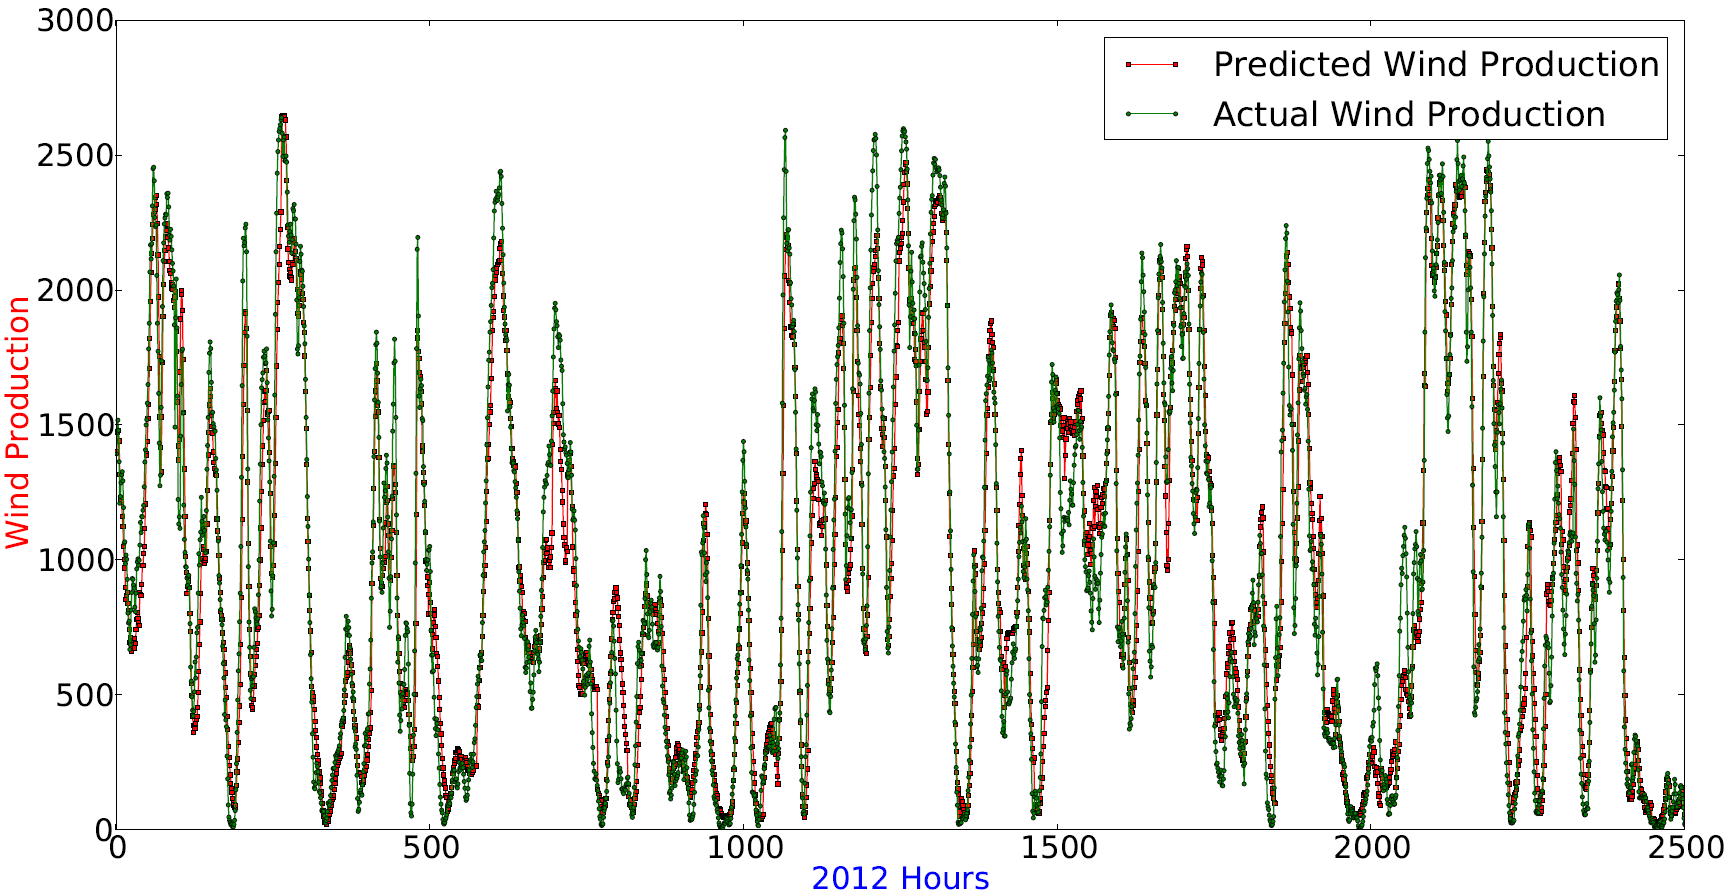
\includegraphics[width=0.99\linewidth]{billeder/bestInputCombi0-2500.png}
\caption{Wind Power prediction for 0-2500 hours in 2012 with the best combination}
\label{fig:bestInputCombi0-2500}
\end{sidewaysfigure} 

\begin{sidewaysfigure}[h!]
\centering
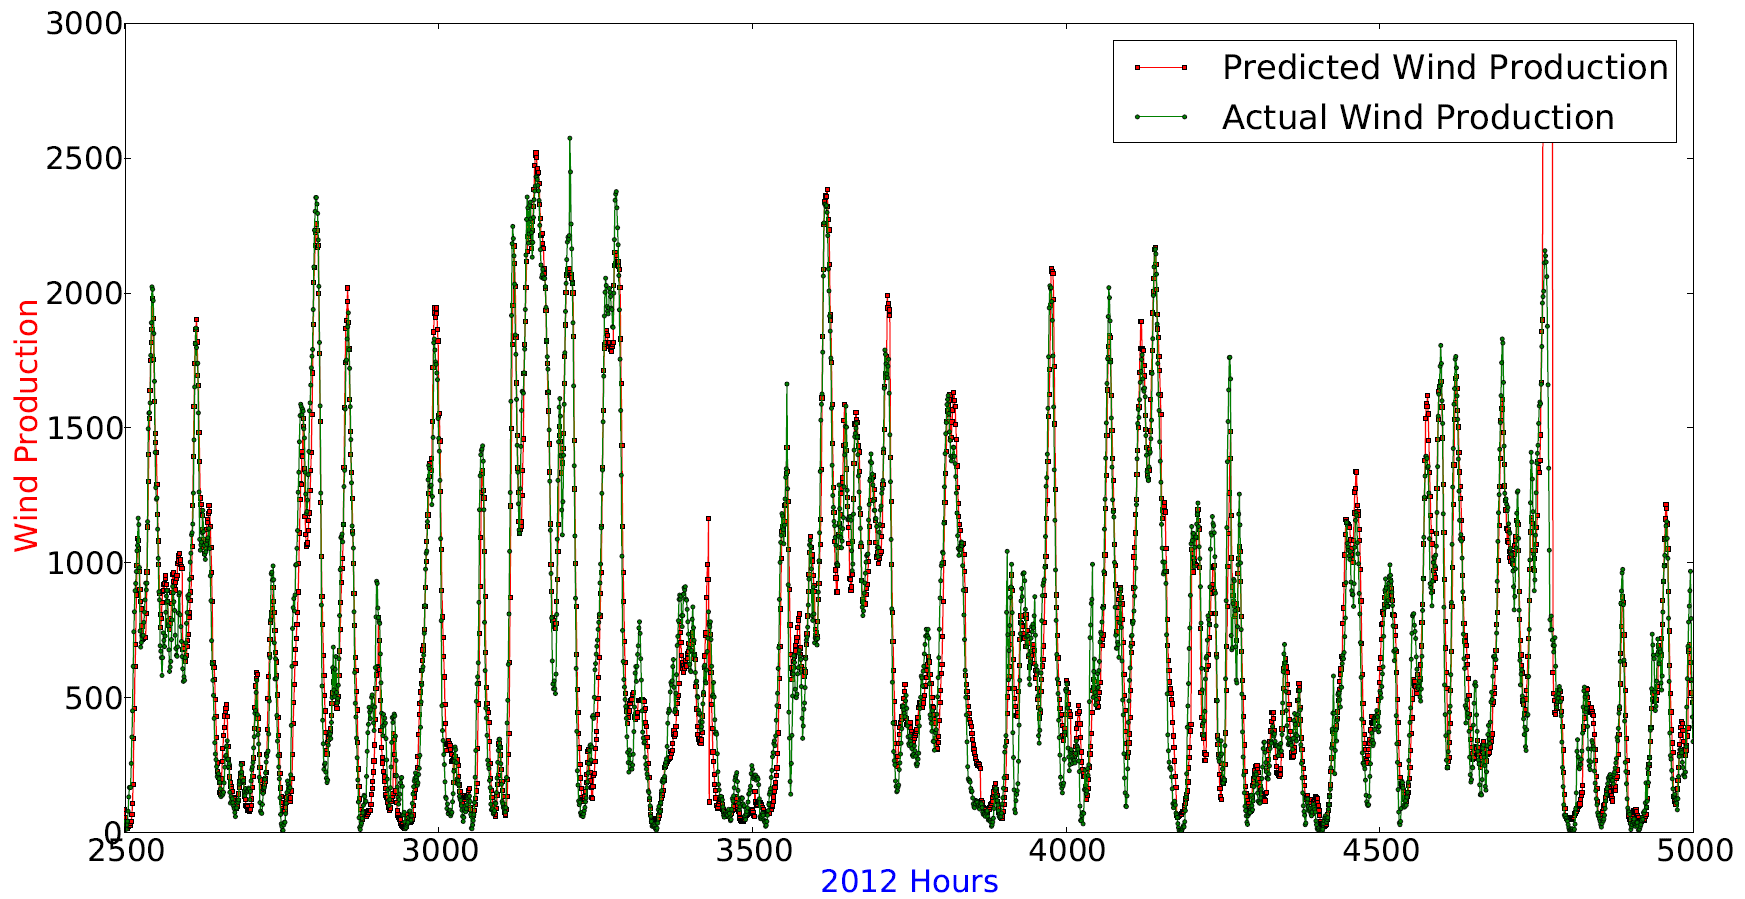
\includegraphics[width=0.99\linewidth]{billeder/bestInputCombi2500-5000.png}
\caption{Wind Power prediction for 2500-5000 hours in 2012 with the best combination}
\label{fig:bestInputCombi2500-5000}
\end{sidewaysfigure} 

\subsection{Experiment Two:}

\subsubsection{Simple input test with seasonality}
\label{sec:simpleInputTestSeason}
The simple input test based on 3 months before the prediction day and the same month in the previous year. All with 200 epochs.

WS = Wind Speed
AD = Air Density
C = Consumption
T = Temperature
WD = Wind Direction
L-P = Last Known Production
D = Date
ToD = Time of Day
M = Time of Day as matrix
CD = Correct direction in \%

\footnotesize
\begin{center}
\begin{longtable}{|c|c|c|c|c|c|c|c|c|c|c|c|c|}
\caption{Wind Production Input Parameter Test}\\
\hline
\textbf{WS} & \textbf{AD} & \textbf{C} & \textbf{T} & \textbf{WD} & \textbf{L-P} & \textbf{D}& \textbf{ToD} & \textbf{MAE} & \textbf{\% from \#1} & \textbf{H1} & \textbf{H2} & \textbf{H2} \\
\hline
\endfirsthead
\multicolumn{13}{c}%
{\tablename\ \thetable\ -- \textit{Continued from previous page}} \\
\hline
\textbf{WS} & \textbf{AD} & \textbf{C} & \textbf{T} & \textbf{WD} & \textbf{L-P} & \textbf{D}& \textbf{ToD} & \textbf{MAE} & \textbf{\% from \#1} & \textbf{H1} & \textbf{H2} & \textbf{CD} \\
\hline
\endhead
\hline \multicolumn{13}{r}{\textit{Continued on next page}} \\
\endfoot
\hline
\endlastfoot
\arrayrulecolor{light-gray}
 \x &  \x &  \x &  &  \x &  \x &  &  \x & 142,88 & 0,0\% & 7 & 17 & 73\% \\ \hline
 \x &  &  &  \x &  \x &  \x &  &  \x & 142,89 & 0,01\% & 14 & 11 & 73\% \\ \hline
 \x &  \x &  &  &  \x &  \x &  &  \x & 143,37 & 0,34\% & 3 & 21 & 73\% \\ \hline
 \x &  \x &  \x &  \x &  \x &  \x &  &  \x & 143,97 & 0,76\% & 4 & 25 & 72\% \\ \hline
 \x &  &  &  &  &  \x &  &  \x & 143,98 & 0,77\% & 2 & 21 & 72\% \\ \hline
 \x &  \x &  \x &  \x &  &  \x &  \x &  \x & 144,11 & 0,86\% & 1 & 17 & 73\% \\ \hline
 \x &  \x &  &  &  &  \x &  &  \x & 144,12 & 0,87\% & 7 & 12 & 73\% \\ \hline
 \x &  &  &  &  &  &  &  \x & 144,28 & 0,98\% & 12 & 17 & 41\% \\ \hline
 \x &  &  \x &  &  \x &  \x &  &  \x & 144,42 & 1,08\% & 11 & 10 & 72\% \\ \hline
 \x &  \x &  &  \x &  \x &  \x &  &  \x & 144,48 & 1,12\% & 1 & 17 & 73\% \\ \hline
 \x &  &  \x &  \x &  &  \x &  &  \x & 144,7 & 1,27\% & 21 & 6 & 72\% \\ \hline
 \x &  \x &  \x &  \x &  &  \x &  &  \x & 144,79 & 1,34\% & 18 & 13 & 72\% \\ \hline
 \x &  &  &  &  &  \x &  &  \x & 144,93 & 1,43\% & 18 & 1 & 73\% \\ \hline
 \x &  &  \x &  \x &  \x &  \x &  \x &  \x & 144,98 & 1,47\% & 14 & 9 & 73\% \\ \hline
 \x &  &  \x &  \x &  &  \x &  \x &  \x & 145,02 & 1,5\% & 18 & 11 & 73\% \\ \hline
 \x &  \x &  \x &  \x &  &  \x &  \x &  \x & 145,19 & 1,62\% & 2 & 15 & 73\% \\ \hline
 \x &  &  &  \x &  &  \x &  \x &  \x & 145,29 & 1,69\% & 13 & 6 & 73\% \\ \hline
 \x &  \x &  &  &  &  &  &  \x & 145,51 & 1,84\% & 1 & 22 & 54\% \\ \hline
 \x &  &  \x &  &  \x &  \x &  &  \x & 145,76 & 2,02\% & 13 & 17 & 73\% \\ \hline
 \x &  \x &  \x &  &  \x &  &  &  \x & 145,79 & 2,04\% & 18 & 9 & 62\% \\ \hline
 \x &  \x &  \x &  &  \x &  \x &  \x &  \x & 145,98 & 2,17\% & 1 & 9 & 73\% \\ \hline
 \x &  &  \x &  &  &  &  &  \x & 145,99 & 2,18\% & 16 & 13 & 64\% \\ \hline
 \x &  &  &  &  \x &  &  &  \x & 146,24 & 2,35\% & 24 & 9 & 61\% \\ \hline
 \x &  \x &  \x &  &  \x &  \x &  &  \x & 146,49 & 2,53\% & 2 & 13 & 72\% \\ \hline
 \x &  &  \x &  &  &  \x &  &  \x & 146,53 & 2,55\% & 1 & 18 & 73\% \\ \hline
 \x &  \x &  \x &  &  &  &  &  \x & 146,57 & 2,58\% & 24 & 11 & 64\% \\ \hline
 \x &  \x &  \x &  &  \x &  \x &  \x &  \x & 146,61 & 2,61\% & 5 & 15 & 72\% \\ \hline
 \x &  \x &  &  \x &  \x &  \x &  \x &  \x & 146,64 & 2,63\% & 1 & 13 & 73\% \\ \hline
 \x &  \x &  \x &  \x &  \x &  \x &  \x &  \x & 146,78 & 2,73\% & 2 & 16 & 73\% \\ \hline
 \x &  \x &  \x &  \x &  \x &  \x &  \x &  \x & 146,89 & 2,81\% & 4 & 16 & 72\% \\ \hline
 \x &  \x &  &  &  &  &  &  \x & 146,96 & 2,86\% & 25 & 5 & 54\% \\ \hline
 \x &  \x &  \x &  &  &  \x &  &  \x & 147,18 & 3,01\% & 14 & 15 & 72\% \\ \hline
 \x &  &  \x &  \x &  &  \x &  &  \x & 147,3 & 3,09\% & 17 & 7 & 72\% \\ \hline
 \x &  &  &  &  &  \x &  \x &  \x & 147,64 & 3,33\% & 11 & 11 & 73\% \\ \hline
 \x &  &  \x &  &  &  &  &  \x & 147,7 & 3,37\% & 11 & 22 & 63\% \\ \hline
 \x &  \x &  \x &  &  &  &  &  \x & 147,86 & 3,49\% & 10 & 25 & 63\% \\ \hline
 \x &  &  &  &  \x &  \x &  \x &  \x & 147,95 & 3,55\% & 4 & 17 & 73\% \\ \hline
 \x &  &  \x &  &  &  \x &  &  \x & 147,98 & 3,57\% & 14 & 17 & 72\% \\ \hline
 \x &  &  &  &  \x &  \x &  \x &  \x & 148,23 & 3,74\% & 1 & 23 & 73\% \\ \hline
 \x &  \x &  &  \x &  &  \x &  \x &  \x & 148,28 & 3,78\% & 5 & 13 & 73\% \\ \hline
 \x &  &  &  \x &  \x &  \x &  \x &  \x & 148,4 & 3,86\% & 13 & 13 & 73\% \\ \hline
 \x &  \x &  &  \x &  &  \x &  &  \x & 148,57 & 3,98\% & 21 & 14 & 72\% \\ \hline
 \x &  \x &  \x &  \x &  &  &  &  \x & 148,66 & 4,05\% & 14 & 20 & 63\% \\ \hline
 \x &  \x &  \x &  \x &  &  &  &  \x & 149,0 & 4,28\% & 7 & 25 & 63\% \\ \hline
 \x &  \x &  &  &  \x &  &  &  \x & 149,04 & 4,31\% & 16 & 12 & 61\% \\ \hline
 \x &  &  &  \x &  &  \x &  &  \x & 149,08 & 4,34\% & 19 & 15 & 72\% \\ \hline
 \x &  &  \x &  &  &  \x &  \x &  \x & 149,13 & 4,37\% & 3 & 16 & 73\% \\ \hline
 \x &  \x &  \x &  &  &  \x &  \x &  \x & 149,28 & 4,48\% & 2 & 16 & 73\% \\ \hline
 \x &  \x &  &  \x &  \x &  \x &  &  \x & 149,31 & 4,5\% & 1 & 17 & 72\% \\ \hline
 \x &  &  \x &  &  \x &  &  &  \x & 149,4 & 4,56\% & 14 & 18 & 63\% \\ \hline
 \x &  \x &  \x &  &  &  \x &  &  \x & 149,95 & 4,95\% & 1 & 16 & 73\% \\ \hline
 \x &  &  \x &  &  \x &  \x &  \x &  \x & 150,28 & 5,18\% & 1 & 22 & 72\% \\ \hline
 \x &  \x &  \x &  \x &  &  \x &  &  \x & 150,33 & 5,21\% & 9 & 19 & 72\% \\ \hline
 \x &  \x &  &  &  &  \x &  \x &  \x & 150,36 & 5,24\% & 4 & 15 & 73\% \\ \hline
 \x &  \x &  &  &  &  \x &  &  \x & 150,98 & 5,67\% & 21 & 1 & 72\% \\ \hline
 \x &  &  &  &  \x &  &  &  \x & 151,09 & 5,75\% & 11 & 21 & 61\% \\ \hline
 \x &  &  \x &  \x &  &  &  &  \x & 151,13 & 5,77\% & 20 & 10 & 63\% \\ \hline
 \x &  &  &  \x &  &  &  &  \x & 151,3 & 5,89\% & 20 & 15 & 50\% \\ \hline
 \x &  \x &  &  \x &  &  \x &  &  \x & 151,45 & 6,0\% & 7 & 20 & 72\% \\ \hline
 \x &  \x &  \x &  \x &  \x &  \x &  &  \x & 151,46 & 6,01\% & 10 & 24 & 72\% \\ \hline
 \x &  \x &  &  &  \x &  \x &  \x &  \x & 151,48 & 6,02\% & 2 & 16 & 73\% \\ \hline
 \x &  \x &  &  \x &  \x &  \x &  \x &  \x & 151,67 & 6,15\% & 4 & 17 & 72\% \\ \hline
 \x &  &  \x &  \x &  &  &  &  \x & 151,7 & 6,17\% & 17 & 13 & 63\% \\ \hline
 \x &  &  \x &  \x &  \x &  \x &  \x &  \x & 151,76 & 6,22\% & 2 & 16 & 72\% \\ \hline
 \x &  &  \x &  \x &  \x &  \x &  &  \x & 151,91 & 6,32\% & 1 & 9 & 71\% \\ \hline
 \x &  &  \x &  \x &  &  \x &  \x &  \x & 152,06 & 6,42\% & 7 & 22 & 72\% \\ \hline
 \x &  \x &  &  &  \x &  &  &  \x & 152,25 & 6,56\% & 19 & 12 & 61\% \\ \hline
 \x &  &  &  &  \x &  \x &  &  \x & 152,28 & 6,58\% & 19 & 14 & 72\% \\ \hline
 \x &  \x &  &  \x &  &  &  &  \x & 152,35 & 6,63\% & 23 & 12 & 54\% \\ \hline
 \x &  \x &  &  &  &  \x &  \x &  \x & 152,36 & 6,63\% & 10 & 22 & 73\% \\ \hline
 \x &  \x &  \x &  \x &  \x &  &  \x &  \x & 152,39 & 6,66\% & 18 & 9 & 63\% \\ \hline
 \x &  &  &  \x &  \x &  \x &  &  \x & 152,43 & 6,68\% & 6 & 23 & 72\% \\ \hline
 \x &  \x &  &  &  \x &  \x &  &  \x & 153,17 & 7,2\% & 2 & 10 & 72\% \\ \hline
 \x &  \x &  \x &  &  &  &  \x &  \x & 153,2 & 7,22\% & 7 & 13 & 63\% \\ \hline
 \x &  &  \x &  \x &  \x &  &  \x &  \x & 153,3 & 7,29\% & 13 & 20 & 63\% \\ \hline
 \x &  &  \x &  \x &  &  &  \x &  \x & 153,52 & 7,45\% & 16 & 15 & 63\% \\ \hline
 \x &  &  &  \x &  &  &  &  \x & 153,6 & 7,5\% & 22 & 14 & 51\% \\ \hline
 \x &  \x &  \x &  &  &  \x &  \x &  \x & 153,82 & 7,66\% & 8 & 14 & 73\% \\ \hline
 \x &  &  \x &  \x &  \x &  &  &  \x & 153,84 & 7,67\% & 9 & 20 & 62\% \\ \hline
 \x &  &  &  &  \x &  \x &  &  \x & 153,95 & 7,75\% & 15 & 12 & 73\% \\ \hline
 \x &  &  \x &  &  \x &  &  &  \x & 154,16 & 7,89\% & 14 & 13 & 61\% \\ \hline
 \x &  \x &  &  \x &  &  &  &  \x & 154,18 & 7,91\% & 12 & 24 & 54\% \\ \hline
 \x &  \x &  \x &  \x &  &  &  \x &  \x & 154,84 & 8,37\% & 13 & 18 & 63\% \\ \hline
 \x &  &  &  \x &  \x &  \x &  \x &  \x & 154,94 & 8,44\% & 1 & 18 & 72\% \\ \hline
 \x &  \x &  \x &  \x &  &  &  \x &  \x & 154,95 & 8,45\% & 2 & 21 & 62\% \\ \hline
 \x &  \x &  &  \x &  &  &  \x &  \x & 155,0 & 8,48\% & 18 & 12 & 54\% \\ \hline
 \x &  &  &  &  &  &  &  \x & 155,07 & 8,53\% & 7 & 21 & 41\% \\ \hline
 \x &  \x &  \x &  &  \x &  &  \x &  \x & 155,46 & 8,8\% & 16 & 15 & 63\% \\ \hline
 \x &  &  \x &  \x &  \x &  &  \x &  \x & 155,7 & 8,97\% & 16 & 18 & 62\% \\ \hline
 \x &  \x &  \x &  \x &  \x &  &  &  \x & 155,79 & 9,04\% & 19 & 11 & 62\% \\ \hline
 \x &  \x &  \x &  &  &  &  \x &  \x & 155,82 & 9,06\% & 7 & 22 & 62\% \\ \hline
 \x &  &  \x &  \x &  &  &  \x &  \x & 155,89 & 9,11\% & 13 & 22 & 63\% \\ \hline
 \x &  \x &  &  &  &  &  \x &  \x & 156,04 & 9,21\% & 22 & 8 & 54\% \\ \hline
 \x &  &  &  \x &  &  \x &  &  \x & 156,14 & 9,28\% & 1 & 21 & 72\% \\ \hline
 \x &  \x &  &  &  \x &  &  \x &  \x & 156,34 & 9,42\% & 14 & 16 & 61\% \\ \hline
 \x &  &  &  \x &  \x &  &  \x &  \x & 156,59 & 9,6\% & 12 & 22 & 61\% \\ \hline
 \x &  &  &  &  &  \x &  \x &  \x & 156,6 & 9,6\% & 22 & 1 & 72\% \\ \hline
 \x &  &  \x &  &  \x &  \x &  \x &  \x & 156,84 & 9,77\% & 1 & 10 & 71\% \\ \hline
 \x &  &  \x &  &  &  &  \x &  \x & 156,89 & 9,81\% & 14 & 19 & 62\% \\ \hline
 \x &  \x &  &  \x &  \x &  &  \x &  \x & 157,48 & 10,22\% & 12 & 17 & 61\% \\ \hline
 \x &  &  &  \x &  &  &  \x &  \x & 157,61 & 10,31\% & 15 & 14 & 50\% \\ \hline
 \x &  &  &  \x &  \x &  &  &  \x & 158,37 & 10,84\% & 25 & 9 & 60\% \\ \hline
 \x &  \x &  &  &  \x &  &  \x &  \x & 158,46 & 10,9\% & 5 & 23 & 61\% \\ \hline
 \x &  \x &  &  \x &  \x &  &  &  \x & 158,64 & 11,03\% & 22 & 9 & 61\% \\ \hline
 \x &  \x &  &  &  &  &  \x &  \x & 158,74 & 11,1\% & 24 & 1 & 54\% \\ \hline
 \x &  \x &  &  &  \x &  \x &  \x &  \x & 159,01 & 11,29\% & 2 & 23 & 72\% \\ \hline
 \x &  &  \x &  &  \x &  &  \x &  \x & 159,25 & 11,46\% & 12 & 23 & 62\% \\ \hline
 \x &  \x &  \x &  \x &  \x &  &  \x &  \x & 159,32 & 11,51\% & 14 & 24 & 62\% \\ \hline
 \x &  \x &  \x &  &  \x &  &  \x &  \x & 159,44 & 11,59\% & 14 & 12 & 63\% \\ \hline
 \x &  &  \x &  &  &  \x &  \x &  \x & 159,6 & 11,7\% & 2 & 13 & 71\% \\ \hline
 \x &  \x &  \x &  &  \x &  &  &  \x & 159,74 & 11,8\% & 12 & 14 & 61\% \\ \hline
 \x &  &  &  \x &  &  &  \x &  \x & 159,94 & 11,94\% & 11 & 15 & 51\% \\ \hline
 \x &  \x &  &  \x &  &  \x &  \x &  \x & 160,11 & 12,06\% & 10 & 14 & 71\% \\ \hline
 \x &  \x &  \x &  \x &  \x &  &  &  \x & 160,55 & 12,37\% & 15 & 19 & 62\% \\ \hline
 \x &  &  &  &  \x &  &  \x &  \x & 160,79 & 12,53\% & 17 & 13 & 61\% \\ \hline
 \x &  &  &  &  &  &  \x &  \x & 160,98 & 12,67\% & 10 & 21 & 41\% \\ \hline
 \x &  \x &  &  \x &  \x &  &  \x &  \x & 161,12 & 12,77\% & 13 & 13 & 61\% \\ \hline
 \x &  &  &  &  &  &  \x &  \x & 161,18 & 12,81\% & 18 & 12 & 41\% \\ \hline
 \x &  &  \x &  &  &  &  \x &  \x & 161,25 & 12,86\% & 3 & 25 & 62\% \\ \hline
 \x &  &  \x &  \x &  \x &  &  &  \x & 161,5 & 13,03\% & 18 & 17 & 62\% \\ \hline
 \x &  &  &  &  \x &  &  \x &  \x & 161,59 & 13,09\% & 16 & 20 & 60\% \\ \hline
 \x &  \x &  &  \x &  &  &  \x &  \x & 162,1 & 13,45\% & 6 & 22 & 54\% \\ \hline
 \x &  &  \x &  &  \x &  &  \x &  \x & 162,54 & 13,76\% & 12 & 13 & 62\% \\ \hline
 \x &  \x &  &  \x &  \x &  &  &  \x & 162,55 & 13,77\% & 19 & 15 & 60\% \\ \hline
 \x &  &  &  \x &  &  \x &  \x &  \x & 162,57 & 13,78\% & 4 & 23 & 71\% \\ \hline
 \x &  &  &  \x &  \x &  &  &  \x & 162,87 & 13,99\% & 15 & 19 & 60\% \\ \hline
 \x &  &  &  \x &  \x &  &  \x &  \x & 163,34 & 14,32\% & 15 & 19 & 61\% \\ \hline
 \x &  &  \x &  \x &  \x &  \x &  &  \x & 165,37 & 15,74\% & 13 & 18 & 71\% \\ \hline
\end{longtable}
\label{table:windProdInputParamsSeasonal}
\end{center}
\normalsize

\subsubsection{Historical volatility results}
\label{sec:historicalVolatiltiyResultsAppendix}
Historical volatility results with all combinations of previous hours between 4-24 and different smoothing factors.

\footnotesize
\begin{center}
\begin{longtable}{|c|c|c|c|}
\caption{Wind Production Input Parameter Test}\\
\hline
\textbf{Previous Hours} & \textbf{Smoothing factor} & \textbf{MAE} & \textbf{\% Deviation} \\
\hline
\endfirsthead
\multicolumn{4}{c}%
{\tablename\ \thetable\ -- \textit{Continued from previous page}} \\
\hline
\textbf{Previous Hours} & \textbf{Smoothing factor} & \textbf{MAE} & \textbf{\% Deviation} \\
\hline
\endhead
\hline \multicolumn{4}{r}{\textit{Continued on next page}} \\
\endfoot
\hline
\endlastfoot
\arrayrulecolor{light-gray}
6 & 0,70 & 121,81 & 0,0\% \\ \hline
20 & 0,80 & 122,9 & 0,89\% \\ \hline
24 & 0,60 & 123,13 & 1,08\% \\ \hline
24 & 0,80 & 124,02 & 1,81\% \\ \hline
16 & 0,20 & 125,65 & 3,15\% \\ \hline
12 & 0,30 & 127,0 & 4,26\% \\ \hline
24 & 0,70 & 127,06 & 4,31\% \\ \hline
16 & 0, 60 & 127,38 & 4,57\% \\ \hline
24 & 0,40 & 127,51 & 4,68\% \\ \hline
16 & 0,90 & 127,77 & 4,89\% \\ \hline
16 & 0,30 & 127,86 & 4,97\% \\ \hline
4 & 0,60 & 128,49 & 5,48\% \\ \hline
4 & 0,10 & 128,51 & 5,5\% \\ \hline
20 & 0,50 & 129,36 & 6,2\% \\ \hline
8 & 0,10 & 130,06 & 6,77\% \\ \hline
24 & 0,20 & 131,05 & 7,59\% \\ \hline
12 & 0,90 & 131,87 & 8,26\% \\ \hline
20 & 0,10 & 132,63 & 8,88\% \\ \hline
20 & 0,30 & 133,32 & 9,45\% \\ \hline
6 & 0,20 & 133,67 & 9,74\% \\ \hline
4 & 0,30 & 133,84 & 9,88\% \\ \hline
12 & 0,60 & 134,02 & 10,02\% \\ \hline
4 & 0,20 & 134,18 & 10,16\% \\ \hline
16 & 0,40 & 134,28 & 10,24\% \\ \hline
4 & 0,40 & 134,71 & 10,59\% \\ \hline
12 & 0,40 & 135,05 & 10,87\% \\ \hline
16 & 0,80 & 135,14 & 10,94\% \\ \hline
20 & 0,20 & 135,3 & 11,07\% \\ \hline
12 & 0,50 & 135,42 & 11,17\% \\ \hline
24 & 0,90 & 135,71 & 11,41\% \\ \hline
16 & 0,50 & 136,44 & 12,01\% \\ \hline
4 & 0,50 & 136,58 & 12,13\% \\ \hline
6 & 0,30 & 136,6 & 12,14\% \\ \hline
20 & 0,70 & 136,63 & 12,17\% \\ \hline
20 & 0,60 & 136,86 & 12,36\% \\ \hline
12 & 0,20 & 136,98 & 12,45\% \\ \hline
6 & 0,10 & 137,16 & 12,6\% \\ \hline
24 & 0,10 & 137,34 & 12,75\% \\ \hline
6 & 0,50 & 137,45 & 12,84\% \\ \hline
24 & 0,50 & 137,91 & 13,22\% \\ \hline
20 & 0,90 & 137,92 & 13,23\% \\ \hline
8 & 0,20 & 138,26 & 13,5\% \\ \hline
8 & 0,40 & 138,69 & 13,86\% \\ \hline
6 & 0,60 & 138,87 & 14,01\% \\ \hline
8 & 0,50 & 138,93 & 14,05\% \\ \hline
8 & 0,60 & 139,2 & 14,28\% \\ \hline
8 & 0,90 & 139,84 & 14,8\% \\ \hline
8 & 0,70 & 140,01 & 14,94\% \\ \hline
24 & 0,30 & 140,45 & 15,3\% \\ \hline
6 & 0,70 & 141,3 & 16,0\% \\ \hline
8 & 0,30 & 141,6 & 16,25\% \\ \hline
4 & 0,70 & 142,19 & 16,73\% \\ \hline
12 & 0,80 & 142,2 & 16,74\% \\ \hline
6 & 0,40 & 142,98 & 17,38\% \\ \hline
6 & 0,80 & 143,21 & 17,57\% \\ \hline
20 & 0,40 & 143,59 & 17,88\% \\ \hline
8 & 0,80 & 143,62 & 17,9\% \\ \hline
12 & 0,10 & 144,37 & 18,52\% \\ \hline
16 & 0,70 & 144,43 & 18,57\% \\ \hline
16 & 0,10 & 146,77 & 20,49\% \\ \hline
4 & 0,80 & 146,9 & 20,6\% \\ \hline
6 & 0,90 & 147,48 & 21,07\% \\ \hline
4 & 0,90 & 151,15 & 24,09\% \\ \hline
\end{longtable}
\label{table:historicalVolatilityAppendixTable}
\end{center}
\normalsize